\documentclass[11pt,a4paper]{article}
\usepackage[margin=25mm]{geometry}
\usepackage{amsmath,amssymb,amsthm,booktabs,graphicx,microtype}
\usepackage[colorlinks=true,allcolors=blue]{hyperref}
\usepackage{caption}
\captionsetup{font=small}
\newcommand{\E}{\mathbb E}
\newcommand{\Var}{\operatorname{Var}}
\newcommand{\ind}{\mathbf 1}
\newcommand{\dd}{\mathrm d}
\newtheorem{proposition}{Proposition}
\title{Relation statistics in a vacuum plane-wave diamond:\newline tidal response, dimension bias and window dependence}
\author{Juneyoung Kim\\\small Independent researcher, Seoul, Republic of Korea\\\small\texttt{lpaiu.cs@gmail.com}}
\date{22 September 2026\\\small Research manuscript for author review}
\begin{document}
\maketitle
\begin{abstract}
Ricci-flatness does not remove the finite-diamond curvature response of the
relation fraction. For a four-dimensional constant vacuum plane wave, we
evaluate its mean and shared-event covariance by explicit subinterval-volume
integrals. With unit null-coordinate span and amplitude $A$, these are
$p_D=1/10-23A^2/75600+O(A^4)$ and
$\zeta_D=1/100-211A^2/4158000+O(A^4)$.
The mean, interpreted through the flat Myrheim--Meyer relation, gives
$d_{\rm pop}=4+23A^2/6363+O(A^4)$ although the manifold dimension is four.
This supplies a vacuum benchmark for separating tidal curvature from apparent
dimension change. A normal-coordinate volume calculation agrees with exact
slicing; we also document a coefficient mismatch with a displayed literature
formula. Fixed coordinate boxes provide controlled contrasts: anisotropy permits
linear response, and a square box has the opposite quadratic sign to the diamond.
The standard U-statistic variance connects the calculated moments to
finite-sample detection forecasts. A previously frozen validation on 51,200
independent fixed-size orders supported all eight forecasts at the prescribed
$\pm10$ percentage-point interval resolution, with flat false-positive upper
bounds below 5\%. The diamond confirmation concerns a weak-amplitude control,
not a measured detection transition. Neither a general Weyl estimator nor
an obstruction for the full causal order is established.
\end{abstract}

\section{Question and relation to previous work}
Finite causal orders contain statistical information about the Lorentzian
regions from which they are sampled. Bombelli's finite-$n$ distributions already
provide a framework for comparing geometries in this way~\cite{bombelli}.
Roy, Sinha and Surya~\cite{roy} express chain counts through nested interval
volumes, calculate leading Ricci corrections, and identify shared-event
fluctuations. Kambor and Nomaan~\cite{kambor} study the resulting estimators
numerically. We use these established ingredients. Our question is the explicit
next response in a tractable vacuum geometry: what remains in the mean and noise
when the Ricci terms vanish, and what does that response imply for interpreting
one finite order?

Window choice matters because two operations must be distinguished. Keeping a
coordinate box fixed changes the causal relation at fixed volume measure.
Keeping the tips of an Alexandrov interval fixed also changes its boundary and
normalization. Work on several definitions of small causal diamonds already
demonstrates the importance of the region definition~\cite{wang}.
A volume expansion alone is not the normalized relation probability: the
outer domain and the subinterval orientations must also be integrated.
We evaluate those integrals exactly as low-dimensional representations in a
constant-profile plane wave, including the shared-event covariance.

Recent work proposes Weyl-sensitive Hasse-diagram observables~\cite{alfyorov}
and investigates conditional sampling costs and bulk response channels~\cite{ghosh}.
The paired flat/curved constructions and strata in the former use different
inputs from our test on one order with known sampling protocol. Neither method
is ranked against the other here. Graph observables also discriminate multiple
causal-set ensembles~\cite{eichhorn}. An APS abstract describes plane-wave Weyl
tests through geodesic deviation~\cite{ahmed}; only its abstract was available
for this comparison. We make no claim to the first Weyl detection, an exhaustive
priority search, or reconstruction of an arbitrary curvature tensor.

The proposed contribution is the explicit vacuum-diamond mean and covariance,
their tidal and dimension-calibration consequences, and a comparison with
coordinate windows. The general nested-volume method and the variance identity
are not contributions claimed here. A formula-level comparison also finds a
specific volume-coefficient disagreement with Eq.~(79) of
arXiv:1904.01034v2~\cite{wang}; Appendix~\ref{rnc} supplies two coordinate
calculations and a check of that reference's intermediate expressions.
This is a comparison in one spacetime, not a replacement general formula.
The dimension consequence and this comparison were developed after confirmation;
the independent numerical validation below retains its original forecasts and
verdicts. An earlier exploratory repository programme motivates the work but is
not presented as additional new evidence.

\section{Geometry, populations and information available}
With natural units $c=1$, consider
\begin{equation}
 \dd s^2=2\dd u\dd v+A(x^2-y^2)\dd u^2+\dd x^2+\dd y^2 . \label{metric}
\end{equation}
For constant $A$, the transverse trace vanishes, so $R_{\mu\nu}=0$;
$R_{uxux}=-A$ and $R_{uyuy}=A$ in the usual curvature convention.
The metric determinant is $-1$. Thus nonzero $A$ changes tidal curvature and
causal order while the coordinate volume form remains
$\dd u\dd v\dd x\dd y$. The amplitude is defined in this chosen null frame.
With $\Delta u=1$, its numerical value is the dimensionless parameter
$A(\Delta u)^2$; it is not a frame-independent curvature scalar.

We use $0\leq A\leq2$, before the first conjugate separation
$\sqrt{A}\Delta u=\pi$. All three boxes have $0<u<1$,
$-1/2<v<1/2$, and transverse full widths $(a,b)$ centred on zero:
\begin{equation}
 R_+:(2,6),\qquad R_0:(\sqrt{12},\sqrt{12}),\qquad R_-:(6,2).
\end{equation}
Each has volume 12. The fourth population is the Alexandrov interval $D_A$
between $P=(0,1/2,0,0)$ and $Q=(1,-1/2,0,0)$. The axial tip proper time is
$\sqrt2$ in every arm. Its volume is $\pi/6$ at $A=0$ and changes with $A$.

Each realization contains exactly $N$ independent points from the normalized
physical volume of its region. This is the fixed-$N$ conditional version of
Poisson sprinkling. Independent arms have independent points. The construction
specifies a continuum sampling protocol; it does not infer windows or tips from
an arbitrary unlabelled order. The statistic receives just the order and $N$,
while its threshold is calibrated to the known region and $N$. It receives no
point correspondence, coordinates, or value of $A$ for the tested realization.
Comparisons at fixed $N$ between boxes and diamonds are \emph{not} comparisons
at matched physical density.

For the transitive causal relation, let $h_{ij}=1$ if points $i,j$ are related,
and zero otherwise. We study
\begin{equation}
 f_N={1\over\binom N2}\sum_{i<j}h_{ij},\qquad
 p_R(A)=\E f_N . \label{f}
\end{equation}
These are relations, not only links in the Hasse diagram. Null boundaries have
zero sampling probability, but numerical near-boundary decisions are checked.

\section{Exact causal relation}
Sort a pair by $u$ and set $s=u_q-u_p$, $d_x=x_q-x_p$,
$m_x=(x_p+x_q)/2$, and similarly for $y$. For $w=\sqrt A>0$, the classical
transverse action is
\begin{align}
 C_A={}&w\tanh(ws/2)m_x^2+{w\over4}\coth(ws/2)d_x^2\nonumber\\
       &-w\tan(ws/2)m_y^2+{w\over4}\cot(ws/2)d_y^2 . \label{action}
\end{align}
The pair is causal precisely when $\Delta v+C_A\leq0$. This follows by
minimizing $\tfrac12\int(x'^2+y'^2+A(x^2-y^2))\dd u$ with fixed transverse
endpoints. The transverse equations are $x''=Ax$, $y''=-Ay$; their action is
minimizing in the stated pre-conjugate domain. Equation~\eqref{action} is a
half-angle evaluation of that standard solution, not a new causal law.

\section{Diamond boundary, mean and covariance}\label{diamond}
For $0<t<s$, define
\begin{equation}
 B_x(t;s)={w\over2}[\coth(wt)+\coth(w(s-t))],\quad
 B_y(t;s)={w\over2}[\cot(wt)+\cot(w(s-t))], \label{B}
\end{equation}
and $J(s)=\int_0^s[B_x(t;s)B_y(t;s)]^{-1/2}\dd t$.
Both coefficients are positive in the specified domain. Completing the two
action quadratics about the classical transverse path shows that any subinterval
with $u$ separation $s$ and slack $\ell=-\Delta v-C_A(p,q)>0$ has volume
\begin{equation}
 V(p,q)={\pi\ell^2\over2}J(s). \label{intervalvol}
\end{equation}
Indeed the intermediate transverse ellipse has height
$\ell-B_x\xi^2-B_y\eta^2$ in $v$; its integrated slice is
$\pi\ell^2/(2\sqrt{B_xB_y})$. This argument also explains why fixed coordinate
volume form does not imply fixed Alexandrov volume.

In the main diamond write $S(u)=[B_x(u;1)B_y(u;1)]^{-1/2}$.
The $u$ marginal is $S(u)/J(1)$ and $V(D_A)=\pi J(1)/2$.
At fixed $u$, the squared elliptical radius has density $2(1-r^2)$;
angle is uniform. For width $L=1-r^2$ and
$z=(v-v_{\rm low})/L$, $L$ has density $2L$ and $z$ is independent uniform.
The conditional probability that an independent point is related to $X$ is
\begin{equation}
 q(X)={L^2\over J(1)}[J(u)(1-z)^2+J(1-u)z^2]. \label{degree}
\end{equation}
The past and future subdiamonds lie inside the main diamond, so their normalized
volumes can be added. This is the conditional-volume form of the known chain
and overlap construction, rather than a new identity. Integrating $L,z$ gives
explicit smooth low-dimensional expressions
\begin{align}
 p_D&={1\over6J(1)^2}\int_0^1 S(u)[J(u)+J(1-u)]\dd u,\label{pd}\\
 \E q^2&={1\over J(1)^3}\int_0^1 S(u)
 \left\{{J(u)^2+J(1-u)^2\over15}+{J(u)J(1-u)\over45}\right\}\dd u,\label{qd}\\
 \zeta_D&=\E q^2-p_D^2.\nonumber
\end{align}
At $A=0$, $J(s)=s^2/3$, $p_D=1/10$ and $\zeta_D=1/100$.

\begin{proposition}[Diamond response]
For these fixed axial tips,
\begin{equation}
 p_D={1\over10}-{23\over75600}A^2+O(A^4),\qquad
 \zeta_D={1\over100}-{211\over4158000}A^2+O(A^4). \label{diamondcoeff}
\end{equation}
\end{proposition}
\begin{proof}
Use $\sin z\sinh z/z^2=1-z^4/90+O(z^8)$ in~\eqref{B}. This gives
\begin{align}
 J(s)&={s^2\over3}\left[1+{A^2s^4\over252}+O(A^4)\right],\nonumber\\
 S(u)&=2u(1-u)\left[1+{A^2(1-u^4-(1-u)^4)\over180}+O(A^4)\right].
\end{align}
Substitution into~\eqref{pd}--\eqref{qd} leaves polynomial integrals on
$[0,1]$ and yields~\eqref{diamondcoeff}. Analyticity in $A^2$ follows from
the displayed sine/hyperbolic-sine product and its positive denominator;
the remainder is therefore justified here independently of parity.
\end{proof}
\subsection{Tidal meaning and flat-calibration bias}\label{dimensionbias}
Along the axial geodesic, choose the unit tangent
$U=(\partial_u-\partial_v)/\sqrt2$ and its orthogonal spatial frame.
The electric Weyl tensor $E_{ij}=C(U,e_i,U,e_j)$ has diagonal entries
$(-A/2,A/2,0)$. For tip proper time $T=\sqrt2$, the dimensionless tidal
strength is $\kappa=E_{ij}E^{ij}T^4=2A^2$. Thus
\begin{equation}
 p_D={1\over10}-{23\over151200}\kappa+O(\kappa^2),\qquad
 \zeta_D={1\over100}-{211\over8316000}\kappa+O(\kappa^2).
 \label{tidal}
\end{equation}
This expression retains the diamond's timelike orientation. A single plane-wave
family cannot determine separate coefficients of all Weyl contractions in a
general vacuum metric. Restoring an arbitrary null span $\Delta u$ replaces
$A$ in~\eqref{diamondcoeff} by $A(\Delta u)^2$.

The flat ordering probability in dimension $d$ is
\begin{equation}
 F(d)={\Gamma(d+1)\Gamma(d/2)\over2\Gamma(3d/2)},\quad
 F(4)={1\over10},\quad F'(4)=-{101\over1200}.
\end{equation}
This normalization is twice $\langle C_2\rangle/\langle C_1\rangle^2$
in the Poisson convention of Ref.~\cite{roy}. Let $d_{\rm pop}$ solve
$F(d_{\rm pop})=p_D(A)$ near four. The inverse-function expansion gives
\begin{equation}
 d_{\rm pop}=4+{23\over6363}A^2+O(A^4)
            =4+{23\over12726}\kappa+O(\kappa^2). \label{dimension}
\end{equation}
This is a curvature bias of the \emph{population calibration}; it is not
$\E[F^{-1}(f_N)]$, which has additional nonlinear sampling bias. At the flat
point, the leading standard error of that inverse is
$240/(101\sqrt N)$. Equations~\eqref{tidal}--\eqref{dimension} give a quantitative
vacuum benchmark: a positive apparent dimension shift can arise while the
actual dimension remains four. Curvature bias in dimension estimation is
already known; the result here is its explicit leading coefficient for this
Ricci-flat family. No new Monte Carlo test of this corollary is claimed.

\subsection{Volume consistency check}\label{volumecheck}
The same slice calculation gives
\begin{equation}
 {V(D_A)\over V(D_0)}=1+{A^2\over252}+O(A^4). \label{volumeresult}
\end{equation}
For comparison, the conventions of Ref.~\cite{wang} give
$d=4$, tip half-length $l=T/2=1/\sqrt2$,
$E^2=A^2/2$, $H^2=A^2$ and $D^2=2A^2$.
Substitution into Eq.~(79) of its arXiv v2 PDF yields instead
$1+(43/9450)A^2$ at this order. The coefficient difference is $11/18900$.
It cannot be attributed to a Ricci term or a curvature derivative:
$R_{ab}=0$ and $\nabla R_{abcd}=0$ here. Appendix~\ref{rnc} independently
recovers~\eqref{volumeresult} in normal coordinates. Specializing and
reintegrating that reference's Eqs.~(74),(76) also gives $1/252$.
We report this reproducible disagreement with the displayed final expression;
we have not derived a corrected formula for general vacuum spacetimes or
obtained an external adjudication of the discrepancy.

\section{Coordinate-window contrasts}
In a fixed box, $s$ has density $2(1-s)$ on $(0,1)$. Integrating both independent
uniform $v$ coordinates gives $p_R(A)=\E G(C_A)$, where
\begin{equation}
G(C)=\begin{cases}
1,&C\leq-1,\\
1-(1+C)^2/2,&-1<C<0,\\
(1-C)^2/2,&0\leq C<1,\\
0,&C\geq1.
\end{cases} \label{survival}
\end{equation}
The remaining integral is five-dimensional. It handles negative action as
well as positive action; retaining only the positive branch would lose part
of the finite-amplitude curved population.

\begin{proposition}[Local box coefficients]
For the three boxes above,
$p_R(A)=p_0+c_1A+c_2A^2+o(A^2)$, with the coefficients in
Table~\ref{coefficients} and the exact expressions in Appendix~\ref{exact}.
The identity $p_{(a,b)}(A)=p_{(b,a)}(-A)$ holds when negative $A$ is defined
by exchanging the transverse axes.
\end{proposition}
\begin{proof}
Expanding the action yields $C_A=C_0+AC_1+A^2C_2+O(A^3)$, with
\begin{align}
 C_0&=(d_x^2+d_y^2)/(2s),\nonumber\\
 C_1&=s\{(m_x^2-m_y^2)/2+(d_x^2-d_y^2)/24\},\nonumber\\
 C_2&=-s^3\{(m_x^2+m_y^2)/24+(d_x^2+d_y^2)/1440\}. \label{expansion}
\end{align}
The $A$-dependent derivatives are bounded on these compact boxes, including
as $s\to0$. Since $G'$ is bounded and Lipschitz, dominated convergence applies
to the first and second integrated differences, away from the measure-zero
surfaces $C_0=0,1$. Therefore
\begin{align}
 c_1&=\E[-(1-C_0)C_1\ind_{C_0<1}],\nonumber\\
 c_2&=\E[\{-(1-C_0)C_2+C_1^2/2\}\ind_{C_0<1}]. \label{coeffintegrals}
\end{align}
Conditional on $|d_x|$, the midpoint is uniform on an interval of width
$a-|d_x|$, giving second and fourth moments $(a-|d_x|)^2/12$ and
$(a-|d_x|)^4/80$. Because $\min(a,b)>\sqrt2$, the full displacement disk
$d_x^2+d_y^2<2s$ lies in the support. Polynomial disk integration gives the
listed expressions. Axis exchange gives the identity and $c_1(R_0)=0$.
Finally, both terms of the $c_2$ integrand are nonnegative and their sum is
positive on a set of positive measure.
\end{proof}

\begin{table}[tb]
\centering
\caption{Coefficients in $p_R(A)=p_0+c_1A+c_2A^2+o(A^2)$, derived without
fitting poset samples. The diamond has the stronger $O(A^4)$ remainder.
The equal-volume statement applies to the three boxes only.}
\label{coefficients}
\begin{tabular}{lrrr}\toprule
Region & $p_0$ & $c_1$ & $c_2$\\\midrule
$R_+$ & 0.02380872630 & $+0.04051927709$ & $+0.05074242895$\\
$R_0$ & 0.02454196871 & 0 & $+0.00572728722$\\
$R_-$ & 0.02380872630 & $-0.04051927709$ & $+0.05074242895$\\
$D$ & 0.10000000000 & 0 & $-0.00030423280$\\\bottomrule
\end{tabular}
\end{table}

Evenness alone does not justify an $O(A^4)$ box remainder: $G''$ changes
at zero, and higher differentiability of the integrated expression has not
been established here. All finite-$A$ forecasts use the full integral,
not a Taylor polynomial evaluated outside its controlled local limit.
The diamond and square box have opposite leading quadratic responses.
The box coefficient is about 18.8 times larger in magnitude, but their volumes
and fixed-$N$ noise also differ. This compares the declared protocols,
not all ways of measuring curvature.

\section{Finite-sample forecast and numerical checks}
For independent volume samples, define
$\zeta_R=\E[h_{12}h_{13}]-p_R^2=\Var(\E[h_{12}\mid X_1])$.
Counting overlapping pairs gives the standard U-statistic identity~\cite{hoeffding}
\begin{equation}
 \sigma_R^2(A,N)=\Var(f_N)
 ={2p_R(1-p_R)\over N(N-1)}
  +{4(N-2)\zeta_R\over N(N-1)}. \label{variance}
\end{equation}
Treating the $\binom N2$ relations as independent observations would omit
the second term. Our independent replication unit is the complete order.

For all windows, an additional numerical route evaluates $p_R$ and
$\E[h_{12}h_{13}]$ from three point backbones $(u,x,y)$. Conditional relation
probabilities are clipped affine functions of the anchor's $v$. Their product
is piecewise quadratic and is integrated exactly between breakpoints. The
remaining nine-dimensional integral uses scrambled Sobol points. Final
forecasts used 32 scrambles of $2^{19}$ points per flat/curved region condition,
independent of all poset seeds. Approximate Bonferroni Student intervals for
the moments were propagated through the two normal tails. The largest resulting
probability error allowance was 0.002880. This is numerical error evidence,
not directed-rounding certification or an exact QMC coverage theorem.

The threshold for a known region and $N$ is frozen as the actual two numbers
\begin{equation}
 L_R,U_R=p_R(0)\mp z_{0.995}\sigma_R(0,N).
\end{equation}
A realization is classified as curved if $f_N<L_R$ or $f_N>U_R$.
The forecast is
\begin{equation}
 \widehat\beta_R(A,N)=
 \Phi\!\left({L_R-p_R(A)\over\sigma_R(A,N)}\right)
 +1-\Phi\!\left({U_R-p_R(A)\over\sigma_R(A,N)}\right). \label{forecast}
\end{equation}
Only the variance is exact; the normal distributional approximation needs
validation. No finite-$N$ normal-error theorem is asserted.

The instrument was checked before pilot sampling. Polynomial coefficients
agreed with separate 24- and 40-node Gauss integrations to less than
$2\times10^{-13}$. A numerical geodesic boundary-value solution and independent
action quadrature on 96 prescribed pairs agreed with the analytic action to
maximum scaled discrepancy $1.32\times10^{-13}$. The vector relation evaluator
agreed with the existing scalar predicate on 1,280 prescribed pairs across
five amplitudes, plus boundary cases. Before confirmation, sixteen targeted tests covered permutation
and axis-exchange invariance, conditional integration, chain counting, variance
and interval gates. Two additional artifact-audit tests passed after confirmation.
A symbolic reconstruction reproduced the response coefficients without reading
poset data. A separate post-confirmation audit checked the metric curvature,
normal-coordinate volume and dimension-calibration identities added in this
revision. These computational checks are not external mathematical review.

Diamond sampling uses rejection from the exact $u$ slice density, which is
maximal at $u=1/2$, followed by the elliptical radial and uniform-$v$ draws
above. The maximum follows from concavity of $\log\sin$ and $\log\sinh$.
Tip membership was checked on 4,096 points at each of $A=0,1,2$.
Numerical volumes were 0.5235987756, 0.5256934164 and 0.5321871128.
Only the QMC integration uses a numerical inverse CDF; comparison of 4,097
and 8,193 grid points provided a separate allowance. Actual confirmation samples
do not inherit that discretization. The smooth diamond moments independently
agreed at 32 and 64 Gauss nodes and with the QMC uncertainty intervals.

\section{Prospective validation and results}
A fixed development grid used $A\in\{0,1/64,1/16,1/4,1,2\}$.
The pilot generated 80 independent orders in each region/amplitude condition
at $N=200,800$, for 3,840 orders. Its established $R_+,A=1$ positive control
had positive 95\% difference intervals at both sizes. The pilot was checked
for unexplained mean, variance and tail discrepancies. Compatibility of its
small samples with planning assumptions was not treated as proof of those assumptions.

For each region, the first positive-amplitude grid interval in which the
$N=300$ forecast crossed 50\% supplied its geometric-mean confirmation amplitude.
This selected $A=1/8$ for $R_+,R_-$ and $A=\sqrt2$ for $R_0$.
No crossing occurred in the diamond grid. The prescribed boundary rule
selected $A=1/64$, the nearer positive boundary in forecast probability.
Consequently the diamond confirmation is a weak-signal control; it is not a
strong-amplitude test. Its $A$ was in the pilot, while both confirmation $N$
values and all confirmation seeds were new. The box amplitudes were also new.

At $N=300,1200$, each of eight curved conditions received its own independent
flat arm. The 16 primary binomial intervals use two-sided Clopper--Pearson
construction with error $0.05/16$ per interval, providing at least 95\%
simultaneous sampling coverage for the fixed forecasts. Every flat interval's
upper endpoint must be at most 0.05. Every curved interval, after subtracting
the frozen prediction and expanding by its numerical allowance, must be wholly
inside $[-0.10,0.10]$. A separate detection label requires the curved lower
endpoint to exceed 0.8 and its flat arm to pass. Low detection can therefore
be accurately predicted without satisfying the detection label.

Before pilot data, power scenarios allowed true flat error in
$\{0.01,0.02,0.03\}$ and absolute forecast bias in $\{0,0.02,0.04\}$.
Exact binomial acceptance probabilities and a union bound, with numerical
allowances included, selected $m=3200$ per arm/condition from a fixed ladder.
The worst declared scenario had joint-power lower bound 0.9818, exceeding
the 90\% target. This is conditional design power, not a guarantee when the
true populations violate those scenarios. Protocols, numerical forecasts,
thresholds, seed namespaces and sample sizes were committed before confirmation.
No holdout refitting or optional sample-size extension occurred.

\begin{table}[tb]
\centering\small
\caption{Independent confirmation, $m=3200$ per row per arm. All probabilities
are percentages. Curved CIs and flat upper bounds belong to the common
16-interval, 95\% simultaneous sampling family. All eight prediction-error
intervals also passed after numerical widening. A star marks the separate
80\% detection criterion.}
\label{results}
\begin{tabular}{llrrrrl}\toprule
Region & $N$ & $A$ & Pred. & Obs. & Curved CI & Flat upper\\\midrule
$R_+$ & 300 & 0.125 & 44.84 & 43.53 & [40.94,46.15] & 1.98\\
$R_+$ & 1200 & 0.125 & 98.24 & 98.56 & [97.83,99.11] & 1.72*\\
$R_0$ & 300 & $\sqrt2$ & 66.96 & 66.03 & [63.51,68.49] & 1.72\\
$R_0$ & 1200 & $\sqrt2$ & 99.68 & 99.84 & [99.51,99.97] & 1.64*\\
$R_-$ & 300 & 0.125 & 20.98 & 21.13 & [19.03,23.33] & 1.40\\
$R_-$ & 1200 & 0.125 & 91.91 & 91.56 & [90.01,92.95] & 1.56*\\
$D$ & 300 & 0.015625 & 1.00 & 1.03 & [0.58,1.68] & 1.48\\
$D$ & 1200 & 0.015625 & 1.00 & 1.09 & [0.63,1.75] & 1.52\\\bottomrule
\end{tabular}
\end{table}

\begin{figure}[tb]
\centering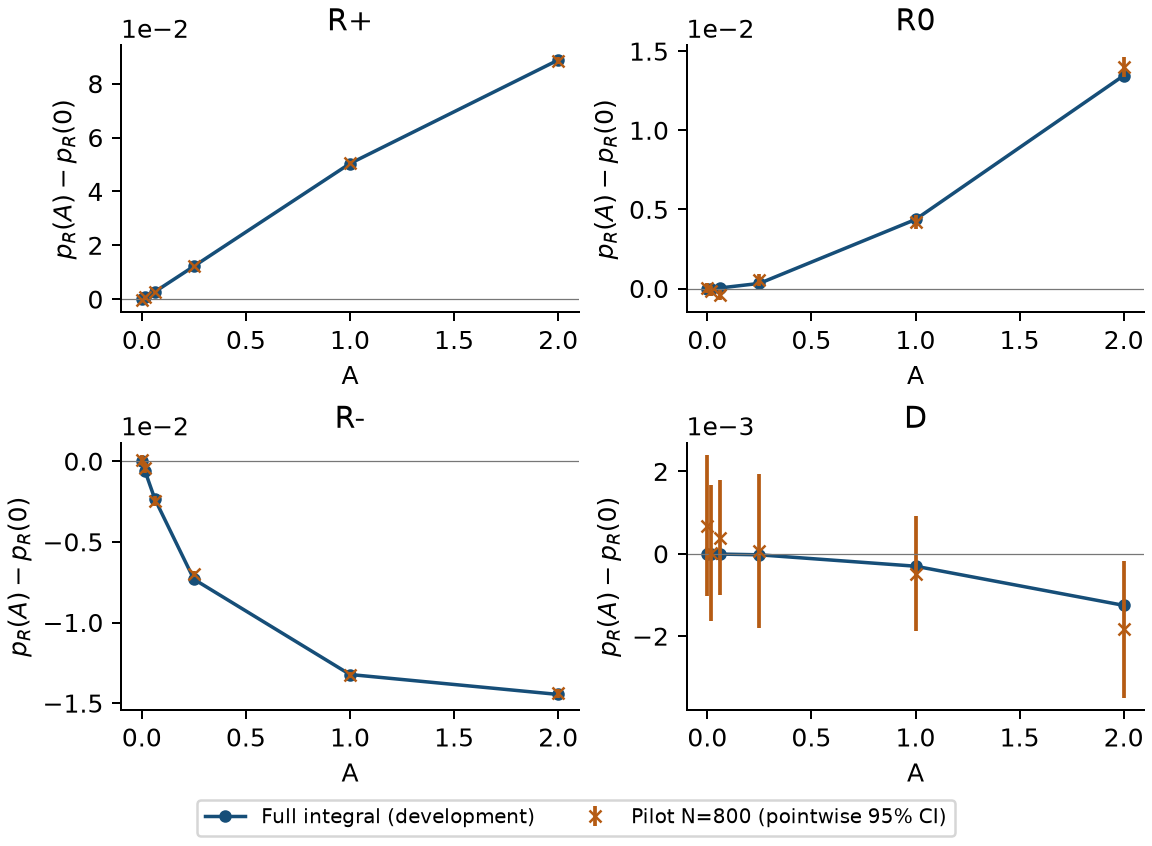
\includegraphics[width=\linewidth]{response.png}
\caption{Mean response at common development amplitudes. Lines connect
quadrature evaluations and are visual guides. Crosses are pilot means with
pointwise 95\% intervals at $N=800$ (80 orders per point). Different vertical
scales are explicit. The noisy diamond pilot does not itself determine the
sign of its weak response; that sign follows from the analytic calculation.}
\label{responsefig}
\end{figure}
\begin{figure}[tb]
\centering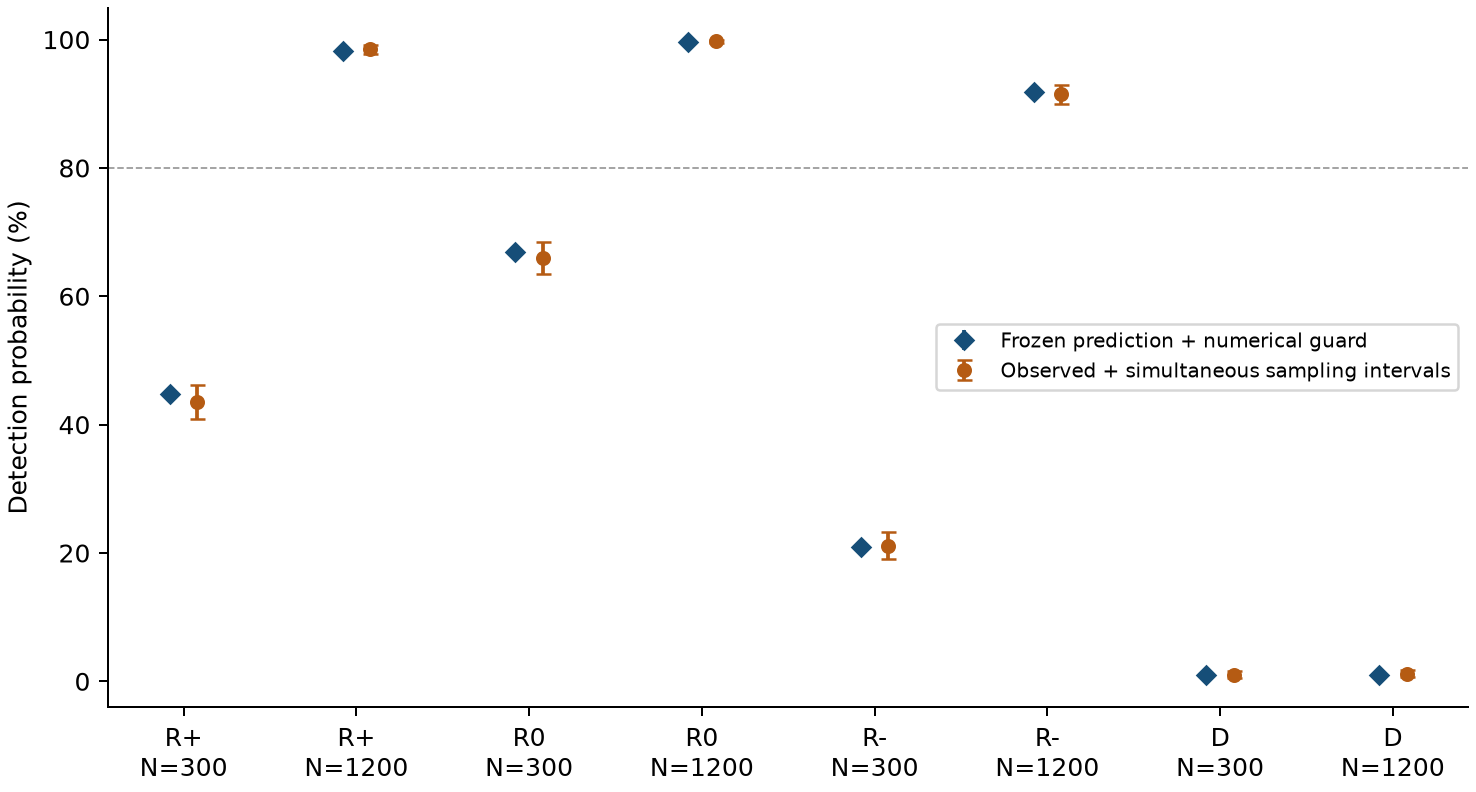
\includegraphics[width=\linewidth]{prediction.png}
\caption{Frozen forecast versus observed detection. Blue guards represent
approximate numerical integration uncertainty; orange intervals represent
simultaneous sampling uncertainty as specified in Table~\ref{results}.
Amplitudes differ by region. The 80\% line is a separate detectability criterion.}
\end{figure}

All 16 gates passed (Table~\ref{results}). The maximum point discrepancy
was 1.31 percentage points. No uncertain pair required precision escalation
in the confirmation data. Absence of such cases in this finite sample does
not prove floating-point correctness on every admissible pair: the guard is
an arithmetic model, and near-guard cases would use the legacy fallback or stop.
An independent audit recomputed counts, intervals and verdicts from the saved
raw statistics and checked their hashes and pre-data forecast commit.

The run used 4,165.05 summed worker CPU seconds and 551.10 wall seconds with
eight workers on the local Windows host. Development grid, pilot and forecast
calculation used 248.31 summed worker CPU seconds, excluding software authoring,
initial instrument checks, process startup and final analysis. The priced
confirmation budget with a factor-two allowance was 1.486 CPU-hours; the
observed 1.157 CPU-hours remained within it and the 48 CPU-hour cap.

\subsection{Secondary comparisons}
The raw data also retain the three-chain fraction
$t_{3,N}=\sum_j d^-_j d^+_j/\binom N3$. These counts use the transitive
relation. Descriptive signed AUCs were oriented using the nearest development
pilot condition, never the confirmation labels. At $N=300$, the respective
$(f_N,t_{3,N})$ AUCs were $(0.9426,0.9437)$ in $R_+$,
$(0.9673,0.9990)$ in $R_0$, and $(0.9157,0.8694)$ in $R_-$.
Thus the extra statistic did not uniformly improve empirical ranking. This
post-confirmation comparison has no simultaneous advantage claim and does
not replace the primary $f_N$ gate. Both statistics were near chance in the
weak diamond condition; noisy pilot orientation there varied with sample size.

Reusing the frozen $R_+$ threshold without region recalibration gave 100\%
flat false positives in both diamond samples. The flat means already explain
this failure ($0.02381$ versus $0.1$); it is not evidence that curvature itself
caused the transfer failure. In $R_0$ at $N=1200$, transferred flat error was
3.25\%, versus 1.00\% under its own calibration. Differences between curved
regions additionally involve different selected $A$ and cannot isolate shape alone.
One balanced random-label diagnostic per condition gave AUCs 0.487--0.509.
It is a diagnostic, not a new hypothesis test.

On a separate $R_0,A=1$ timing sample, nine warm repeats gave median additional
three-chain aggregation times of 0.094 ms at $N=300$ and 1.319 ms at $N=1200$,
after the relation matrix already existed. Matrix construction took 1.948 ms
and 54.258 ms respectively. This small host-specific benchmark measures the
incremental count, not a portable hardware performance bound.

\section{Interpretation and limits}
The diamond calculation identifies an explicit vacuum response beyond the
leading Ricci correction used in small-diamond chain formulae. Its practical
use is as a benchmark for mean, noise and flat-dimension calibration, with a
known geometry and orientation. The volume comparison in Section~\ref{volumecheck}
is also a testable consistency question for higher-order diamond expansions.
Neither result establishes a universal curvature reconstruction procedure.

The quantitative distinction is between the same order statistic under
different acquisition protocols. In the anisotropic boxes, the two transverse
tidal contributions are weighted differently and leave opposite nonzero linear
coefficients. Equal widths cancel that term. In the moving diamond, the
boundary and its normalization enter the response along with the relation;
the resulting quadratic coefficient has the opposite sign.

When $\zeta_R(0)>0$, equation~\eqref{variance} gives standard deviation
asymptotic to $2\sqrt{\zeta_R(0)/N}$. A nonzero local mean response $cA^k$
therefore suggests $A$ of order $N^{-1/(2k)}$ at fixed standardized signal.
This is a standard conditional asymptotic consequence, not a newly measured
scaling law. Two confirmation sizes and moderate box amplitudes do not establish
its asymptotic exponent. Nor can the diamond's weak-amplitude result exclude
information in higher chains or the full order, establish non-detectability
at $A=2$, or prove a universal lower bound on sample complexity.

The successful forecasts support the declared ten-percentage-point resolution
at eight selected conditions. They do not certify exact 1\% tail calibration:
the formal flat upper bound was 5\%. The numerical guards are approximate;
the exact simultaneous sampling statement concerns the frozen numerical
forecast values. We do not combine these into an exact 95\% joint guarantee
over an ideal continuum forecast. Extension beyond the pre-conjugate plane
wave, to other windows, or to inference of unknown window geometry requires
new derivations and independent validation.

\section*{Data, code and declarations}
The companion source, all 51,200 raw statistic triples, development outputs,
protocols, frozen forecasts, validation audit and figure generator accompany
this local review manuscript. The project repository is
\url{https://github.com/lpaiu-cs/causal-spacetime}; the new study is on the local
\texttt{codex/observation-window-response} branch. A public archive of this
study has not yet been deposited. The companion README records producer
commits, hashes, software versions and reproduction commands. Earlier frozen
results and the earlier submission have not been overwritten.

No external research funding was received. The author declared no competing
interests. AI assistance was substantial: OpenAI Codex assisted with literature
comparison, derivations, code, execution, checks and manuscript preparation.
Earlier reused research infrastructure was developed with Anthropic Claude
assistance. AI systems are not authors. The checks reported above are automated
mathematical and numerical checks, not a claim of independent human peer review.
This draft is provided for the named author's review and responsibility before
any new submission.

\appendix
\section{Normal-coordinate volume cross-check}\label{rnc}
This derivation is independent of the conditional-degree calculation and was
added after the frozen campaign. At the axial midpoint use normal coordinates
$(t,z,X,Y)$, put $s=(t+z)/\sqrt2$, and set $w=\sqrt A$.
The exponential map obtained from the geodesic equations is
\begin{align}
 u&=u_O+s,\qquad
 x=X{\sinh(ws)\over ws},\qquad y=Y{\sin(ws)\over ws},\nonumber\\
 v&={-t+z\over\sqrt2}
 -{X^2\over2s}\left({\sinh(ws)\cosh(ws)\over ws}-1\right)\nonumber\\
 &\hspace{12mm}
 -{Y^2\over2s}\left({\sin(ws)\cos(ws)\over ws}-1\right). \label{expmap}
\end{align}
Continuous limits are understood at $s=0$. The absolute Jacobian is
\begin{equation}
 \sqrt{-g_{\rm RNC}}={\sinh(ws)\sin(ws)\over (ws)^2}
 =1-{A^2(t+z)^4\over360}+O(A^4s^8). \label{rncjac}
\end{equation}
The tips have normal times $\pm l$. For the upper cone let $r_0=l-t$,
$(X,Y,z)=r(n_x,n_y,n_z)$ and $d_n=n_x^2-n_y^2$.
Substituting~\eqref{expmap} in the exact null condition and solving gives
\begin{align}
 r&=r_0(1+Ab_1+A^2b_2+O(A^3)),\nonumber\\
 b_1&=-{l^2d_n\over12},\nonumber\\
 b_2&={l^4d_n^2\over96}
 +{l^2(1-n_z^2)\over360}
       [(t+r_0n_z)^2-4l(t+r_0n_z)+l^2]. \label{rncboundary}
\end{align}
The lower cone gives the same integrated contribution. Its moving join with
the upper cone does not change the $A^2$ coefficient: the first-order time
shift is zero and the unperturbed densities agree at the join.
Using normalized angular averages
$\langle d_n^2\rangle=4/15$,
$\langle1-n_z^2\rangle=2/3$ and
$\langle(1-n_z^2)n_z^2\rangle=2/15$, one obtains
\begin{align}
 [A^2]V={}&8\pi\int_0^l\left[
 r_0^3\langle b_2+b_1^2\rangle
 -{1\over360}\left({t^4r_0^3\over3}
                   +{2t^2r_0^5\over5}+{r_0^7\over35}\right)\right]\dd t
 ={2\pi l^8\over189}. \label{rncvolume}
\end{align}
Here $[A^2]$ denotes the Taylor coefficient. Since $V_0=2\pi l^4/3$,
the relative correction is $A^2l^4/63$, giving $A^2/252$ for $l=1/\sqrt2$.
The overall volume is even and analytic in $A$, as is also manifest in the
exact slice formula.

The companion \path{check_diamond_geometry.py} differentiates the original
metric to verify Ricci-flatness, covariantly constant curvature, the tetrad
contractions, the exponential-map Jacobian and the null residual through
$A^2$. It separately specializes Ref.~\cite{wang}, Eqs.~(74),(76), performs
their angular and radial integrals, and obtains the same coefficient. This
agreement localizes the comparison to the displayed final Eq.~(79), without
proposing a general correction. A 60-digit evaluation of the exact slice at
$A=0.1,0.05,0.025,0.0125$ gives $(V/V_0-1)/A^2$ respectively as
$0.0039685733$, $0.0039683338$, $0.0039682739$ and $0.0039682590$,
approaching $1/252=0.0039682540$.
These are deterministic arithmetic checks, not additional statistical evidence.

\section{Exact box coefficient evaluation}\label{exact}
For nonnegative integers $i,j$ and the powers $k$ used here, set
$h=(i+j+2)/2$, $t=k+h$. Integration over the full displacement disk gives
\begin{equation}
 \int_0^1 2(1-s)s^k\!\int_{d_x^2+d_y^2<2s}|d_x|^i|d_y|^j\dd d_x\dd d_y\dd s
 ={4B((i+1)/2,(j+1)/2)2^h\over(i+j+2)(t+1)(t+2)}. \label{betaidentity}
\end{equation}
To evaluate~\eqref{coeffintegrals}, multiply the midpoint-averaged polynomial
by $(a-|d_x|)(b-|d_y|)/(a^2b^2)$ before using~\eqref{betaidentity}.
For $(a,b)=(2,6)$ this yields
\begin{align}
 p_0&={\pi\over108}+{1\over5184}-{128\sqrt2\over33075},\nonumber\\
 c_1&={\pi\over54}+{1\over540}-{352\sqrt2\over25515},\nonumber\\
 c_2&={1613\pi\over48600}+{16733\over2177280}
       -{1316008\sqrt2\over30405375}.
\end{align}
For $R_-$ only the sign of $c_1$ changes. For the square box,
\begin{align}
 p_0&={\pi\over108}+{1\over5184}-{64\sqrt6\over33075},\nonumber\\
 c_1&=0,\qquad
 c_2={257\pi\over48600}+{73\over435456}-{137204\sqrt6\over30405375}.
\end{align}
These are exact coefficients in the stated local expansion; the finite-amplitude
mean is evaluated with~\eqref{action} and~\eqref{survival}. This distinction is
essential in the square-box confirmation at $A=\sqrt2$.

\begin{thebibliography}{99}
\bibitem{bombelli} L. Bombelli, ``Statistical Lorentzian geometry and the
closeness of Lorentzian manifolds,'' J. Math. Phys. \textbf{41}, 6944--6958 (2000).
\href{https://doi.org/10.1063/1.1288494}{doi:10.1063/1.1288494}.
\bibitem{roy} M. Roy, D. Sinha and S. Surya, ``The Discrete Geometry of a Small
Causal Diamond,'' Phys. Rev. D \textbf{87}, 044046 (2013).
\href{https://doi.org/10.1103/PhysRevD.87.044046}{doi:10.1103/PhysRevD.87.044046}.
\bibitem{kambor} J. Kambor and Nomaan X, ``Manifold Properties from Causal Sets
using Chains'' (2020).
\href{https://doi.org/10.1088/1361-6382/abc8c9}{doi:10.1088/1361-6382/abc8c9};
\href{https://arxiv.org/abs/2007.03835}{arXiv:2007.03835}.
\bibitem{wang} J. Wang, ``Geometry of small causal diamonds,'' Phys. Rev. D
\textbf{100}, 064020 (2019).
\href{https://doi.org/10.1103/PhysRevD.100.064020}{doi:10.1103/PhysRevD.100.064020}.
Equation comparison uses
\href{https://arxiv.org/pdf/1904.01034v2}{arXiv:1904.01034v2}, p.~12,
Eq.~(79), identified by its record as the published version; the publisher's
typeset full text was not accessible in this audit.
\bibitem{alfyorov} D. Alfyorov and I. Shnyukov, ``Weyl Curvature from the Hasse
Diagram: A Parameter-Free Bridge Formula for Causal Sets,'' preprint (2026).
\href{https://inspirehep.net/files/32388edfda552e0b4cfb6697bda66d7b}{INSPIRE-hosted version inspected 21 September 2026}.
\bibitem{ghosh} A. Ghosh, ``Sample-Complexity Bounds and an Exact Bulk-Sector
Channel Obstruction for Curvature Estimation on Finite Causal Sets,'' version 4,
preprint (14 August 2026).
\href{https://zenodo.org/records/21931074}{Zenodo record 21931074}.
\bibitem{eichhorn} A. Eichhorn, H. Mack, K. T. Le and F. Wagner,
``Charting causal set configuration space with graph observables,'' preprint
(2026). \href{https://arxiv.org/abs/2605.27514}{arXiv:2605.27514}.
\bibitem{ahmed} S. N. I. Ahmed and L. Bombelli, ``Indications of Weyl curvature in a causal
set,'' APS Global Physics Summit (2026), abstract.
\href{https://meetings-archive.aps.org/smt/2026/apr-r93/1/}{Presentation APR-R93.1}.
\bibitem{hoeffding} W. Hoeffding, ``A Class of Statistics with Asymptotically
Normal Distribution,'' Ann. Math. Statist. \textbf{19}, 293--325 (1948).
\href{https://doi.org/10.1214/aoms/1177730196}{doi:10.1214/aoms/1177730196}.
\end{thebibliography}
\end{document}
